%
% File: chap06.tex
%
\let\textcircled=\pgftextcircled
\chapter{Functional analyses}
\label{chap:fm}

\newacronym{fbed}{FBED}{Functional Basis for Engineering Design}
\newacronym{ffip}{FFIP}{Funtion Failure Identification and Propagation}
\newacronym{ffdm}{FFDM}{Function Failure Design Method}
\newacronym{uffsr}{UFFSR}{Uncoupled Flow Failure State Reasoning}
\newacronym{fsl}{FSL}{Function State Logic}
\newacronym{phm}{PHM}{Prognostic and Health Management}
\newacronym{sta}{STA}{Success Tree Analysis}
\newacronym{hra}{HRA}{Human Reliability Assessment}

\initial{A} different way of representing an engineering system is to embed it as a functional model. A functional model is a graphical representation of a system, that ties a component to a function, or a set of functions, fulfilled within the system. Function are interconnected by flows. One of the main advantage of functional modeling is its applicability in the early stages of design, when no components have been selected and the design is just a concept. Until recently, two main methods existed to create a functional method, NIST and the Functional Basis. Each had their own volatile taxonomy, which limited the widespread use of this technique to other ends than system description. Stone and Wood proposed the \gls{fbed}~\cite{stone}, which reconciled sets of function and flows notably with relation to mechanical engineering design nomenclature. This common taxonomy allowed for automatic analysis methods and database maintenance, which paved the way to various risk and reliability methods based on functional models, such as \gls{ffdm}~\cite{stone2005}, \gls{ffip}~\cite{kurtoglu2007}, \gls{uffsr}~\cite{vanbossuyt2014},~\cite{ohalloran2015} of Prognostics-based analysis in early design (\cite{stack2015} and~\cite{lher2016}).


\section{Functional model}

A FBED description of a system uses the reconciled function set and flow set to name the various functions and flows necessary within a system. Tables~\ref{tab:fbed_func} and~\ref{tab:fbed_flow} give a few example of such functions and flows. FBED is organized using three classes, primary, secondary and tertiary, each increasing the degree of specification. THose three classes cover every potential function seen in a mechanical design. It is to be noted that it still allow for some level of interpretation as to how to categorize a function or flow.

A FBED model can be compared to a RBD. They both can take various degrees of details, high-level to low-level model description. One of the advantages that FBED exhibits as opposed to RBD is that it considers explicitely the flows linking the different functions. Moreover, it does not depend on the component selection, which allow the design team to explore a larger space of possible systems. Figure~\ref{fig:fbed} show an example of a functional model applied to the present case study. One can note that the level of details can be modified. Moreoever, to simplify the drawing, the redundancies displayed by the system are not explicited as separate functions and flows. They are instead encoded within the probabilities associated with each function or flow failure propagation.

\renewcommand{\arraystretch}{1.2}
\begin{table}[t] \small
\centering
\caption{Excerpt from the functional basis reconciled function set}
\label{tab:fbed_func}
\begin{tabular}{|c|c|c|}
\hline
Class (primary)          & Secondary                 & Tertiary  \\ \hline
\multirow{4}{*}{Branch}  & \multirow{3}{*}{Separate} & Divide    \\ \cline{3-3} 
                         &                           & Extract   \\ \cline{3-3} 
                         &                           & Remove    \\ \cline{2-3} 
                         & Distribute                &           \\ \hline
\multirow{7}{*}{Channel} & Import                    &           \\ \cline{2-3} 
                         & Export                    &           \\ \cline{2-3} 
                         & \multirow{2}{*}{Transfer} & Transport \\ \cline{3-3} 
                         &                           & Transmit  \\ \cline{2-3} 
                         & \multirow{3}{*}{Guide}    & Translate \\ \cline{3-3} 
                         &                           & Rotate    \\ \cline{3-3} 
                         &                           & Allow DOF \\ \hline
\multicolumn{3}{|c|}{...}                                        \\ \hline
Support & Position &           \\ \hline
\end{tabular}
\end{table}

\begin{table}[t] \small
\centering
\caption{Excerpt from the functional basis reconciled flow set}
\label{tab:fbed_flow}
\begin{tabular}{|c|c|c|}
\hline
Class (primary)              & Secondary                    & Tertiary                         \\ \hline
\multirow{6}{*}{Material}    & Human                        &                                  \\ \cline{2-3} 
                             & Gas                          &                                  \\ \cline{2-3} 
                             & Liquid                       &                                  \\ \cline{2-3} 
                             & \multirow{3}{*}{Solid}       & Object                           \\ \cline{3-3} 
                             &                              & \multicolumn{1}{l|}{Particulate} \\ \cline{3-3} 
                             &                              & \multicolumn{1}{l|}{Composite}   \\ \hline
\multicolumn{3}{|c|}{...}                                                                      \\ \hline
Energy & Thermal &             \\ \hline
\end{tabular}
\end{table}

\begin{figure}[H]
\centering
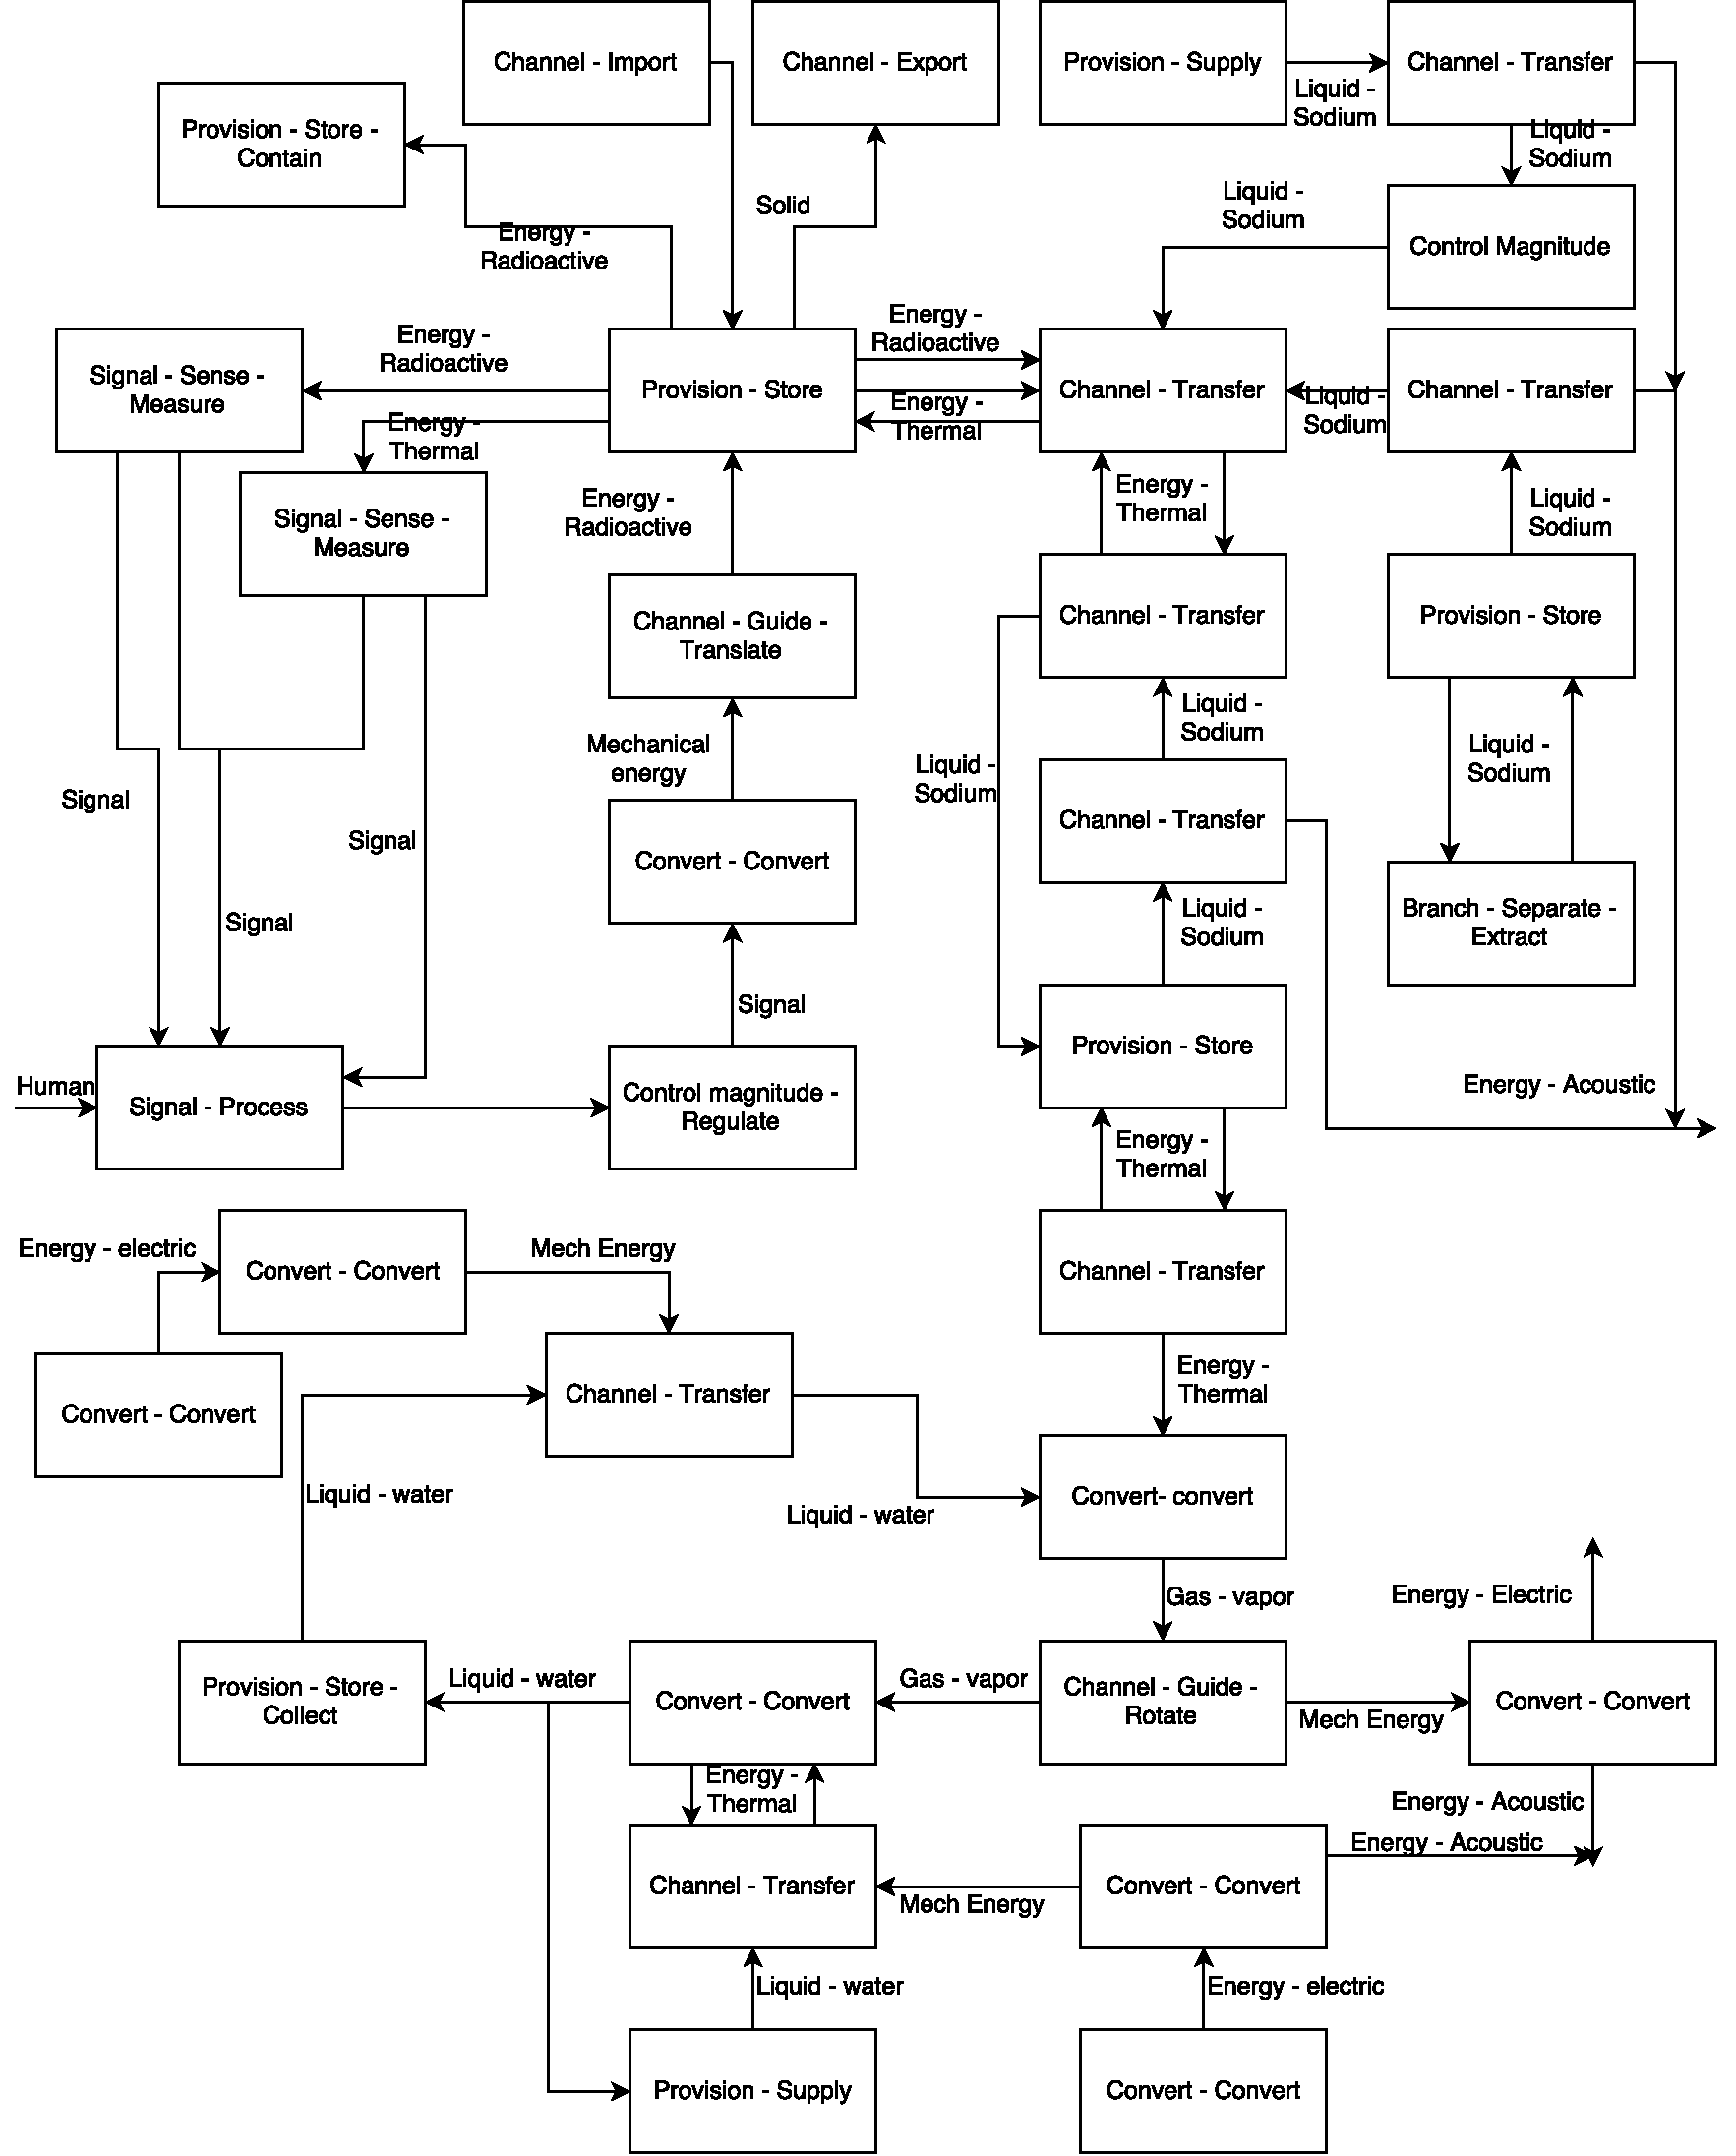
\includegraphics[scale=.6]{fig/Functional_model}
\caption{High-level simplified FBED representation of ASTRID reactor.}
\label{fig:fbed}
\end{figure}

\section{Function Failure Design Method}

FFDM is a method whose main goal is to look at historical component failure data within a system, and estimate the different failure mode observed. Those failure modes are then linked to the functions in the design. Effectively, FFDM is similar to FMEA, but allow for a more generalized approach by taking on functions. The failure modes identified can then be mitigated by modifying the functions used in the system. It has been shown that given the right database available, FFDM gave more information on the potential risk and possible actions to mitigate them in a system than FMEA. Moreover, being based on functions-failure-modes database, this method is less likely to depend uniquely on expert opinion.

However, FFDM does not diagnose the root cause of a failure, nor does it take into account manufacturing and operating conditions. Indeed, FFDM does not differentiate various levels of stress durin operations and is very dependent on past operation data to derive information about failure modes. More importantly, FFDM does not consider the severity or the detectability of a failure mode. It only focuses on the likelihood of a failure mode for each function in the system. This is an important limitation of the methodology, since it doesn't allow the design team to make fully informed decisions.

To illustrate this method, let us assume that a repository of failure modes for a given system is available. An engineering team wants to improve upon the original design, or create a new design entirely. The first step is to translate the system to a functional black-box model. Then, for each function, the failure history is analyzed, and a susceptibility score is used to link a function to all potential failure mode. Given that information, a mitigation analysis is conducted, allowing to choose the most adequate components addressing the identified function failure modes.

The fact that this method is based upon functional model allow for its use in conceptual design. One of its limitation is the existence of a complete database, and the fact that a function can fail following different failure modes depending on operating stresses and component physical attributes.

Table~\ref{tab:ffdm_dat} shows several failure modes occurences for a subset of the case study system functions.

One of the main difficulty of the FFDM method is to populate the database. Historical data is scarcely available for components, and those components must be decomposed into a functional model in order to link failure modes and functions. The failure modes considered should be drawn from a similar system, in terms of operating range and flows, to the system being analyzed. Indeed, a function "Channel - Transfer" would exhibit very different score for each failure mode in a system in which the flow is a potent acid versus a system in which the flow is room temperature water.

In order to compute the data needed for the FFDM analysis, in the absence of meaningful historical data, the FMEA analysis results presented in Table~\ref{tab:fmea_rpn_risk} are considered. Each component was analyzed and a list of potential failure and their likelihood was obtained. The number of occurences is then computed into Table~\ref{tab:ffdm_dat}. Table~\ref{tab:ffdm_norm} presents the normalized data, computed using Equation~\ref{eq:norm}.

\begin{equation}
f_{i, n} = \frac{f_i}{\sum_j F_j}
\label{eq:norm}
\end{equation}
Where:
\begin{conditions}
f_{i, n} & Normalized failure score for the mode $i$ \\
f_{i} & Failure score for the mode $i$ \\
\sum_j F_j & Number of functions considered
\end{conditions}

An example of the methodology applied to derive FFDM database from the FMEA analysis rather than historical data is explicited on the component \textit{Fuel assemblies}. A fuel assembly can be translated into a \textit{Provision - Store - Contain} function. FMEA analysis detected five different potential failure modes: a high power peaking factor, a very high power peaking factor, a human mistake (misidentification), wear and a damage to the head. We can categorize those five failure modes into various categories. The high power peaking factors can both be put in the thermal stress category. A human mistake to misidentify a fuel assembly can be categorized as a human attack. Damage to the assembly head can be sorted into the mechanical stress category. Once the main categories are computed, the likelihood of each events are taken from the FMEA analysis and incremented to the total value for each category. In this example, it would mean that \textit{Thermal stress} has a score of 13 ($8+5$), \textit{Human attack} a score of 3, and so on.

Then, the other components exhibiting the function \textit{Provision - Store - Contain}, such as the inner vessel or the core catcher, are analyzed and their failure modes scores are added to their relevant categories.

\begin{table}[t] \tiny
\centering
\caption{FFDM database}
\label{tab:ffdm_dat}
\begin{tabular}{|c|c|c|c|c|l|c|c|c|}
\hline
Function/Failure            & \begin{tabular}[c]{@{}c@{}}Corrosion\\ Fatigue\end{tabular} & \begin{tabular}[c]{@{}c@{}}Human \\ Attack\end{tabular} & \begin{tabular}[c]{@{}c@{}}Thermal\\ Stress\end{tabular} & \begin{tabular}[c]{@{}c@{}}Mechanical\\ Shock\end{tabular} & \multirow{8}{*}{...} & \begin{tabular}[c]{@{}c@{}}Mechanical\\ Stress\end{tabular} & \begin{tabular}[c]{@{}c@{}}Radiation\\ Damage\end{tabular} & \begin{tabular}[c]{@{}c@{}}Electronic\\ Failure\end{tabular} \\ \cline{1-5} \cline{7-9} 
Channel - Transfer          & 18                                                           & 12                                                                   & 0                                                              & 8                                                       &                      & 0      & 6  & 0 \\ \cline{1-5} \cline{7-9} 
Provision - Store - Contain & 10                                                           & 14                                                                   & 13                                                              & 5                                                       &                      & 0      & 11   & 0 \\ \cline{1-5} \cline{7-9} 
Signal - Sense - Measure    & 0                                                           & 0                                                                   & 0                                                              & 0                                                       &                      & 0      & 0   & 33 \\ \cline{1-5} \cline{7-9} 
Convert - Convert           & 17                                                           & 5                                                                   & 0                                                              & 6                                                       &                      & 0      & 4   & 0 \\ \cline{1-5} \cline{7-9} 
Branch - Separate - Extract & 6                                                           & 0                                                                   & 0                                                              & 0                                                       &                      & 0      & 1   & 0 \\ \cline{1-5} \cline{7-9} 
Channel - Guide - Translate & 0                                                           & 0                                                                   & 0                                                              & 5                                                       &                      & 20      & 0   & 0 \\ \cline{1-5} \cline{7-9}
\multicolumn{9}{|c|}{...}                                                                                                                                                                                                                                                                                                    \\ \hline
\end{tabular}
\end{table}


\begin{table}[t] \tiny
\centering
\caption{FFDM normalized database}
\label{tab:ffdm_norm}
\begin{tabular}{|c|c|c|c|c|l|c|c|c|}
\hline
Function/Failure            & \begin{tabular}[c]{@{}c@{}}Corrosion\\ Fatigue\end{tabular} & \begin{tabular}[c]{@{}c@{}}Human \\ Attack\end{tabular} & \begin{tabular}[c]{@{}c@{}}Thermal\\ Stress\end{tabular} & \begin{tabular}[c]{@{}c@{}}Mechanical\\ Shock\end{tabular} & \multirow{8}{*}{...} & \begin{tabular}[c]{@{}c@{}}Mechanical\\ Stress\end{tabular} & \begin{tabular}[c]{@{}c@{}}Radiation\\ Damage\end{tabular} & \begin{tabular}[c]{@{}c@{}}Electronic\\ Failure\end{tabular} \\ \cline{1-5} \cline{7-9} 
Channel - Transfer          & 4.5                                                           & 3                                                                   & 0                                                              & 2                                                       &                      & 0      & 1.5  & 0 \\ \cline{1-5} \cline{7-9} 
Provision - Store - Contain & 2                                                           & 2.8                                                                   & 2.6                                                              & 1                                                       &                      & 0      & 2.2   & 0 \\ \cline{1-5} \cline{7-9} 
Signal - Sense - Measure    & 0                                                           & 0                                                                   & 0                                                              & 0                                                       &                      & 0      & 0   & 16.5 \\ \cline{1-5} \cline{7-9} 
Convert - Convert           & 4.25                                                           & 1.25                                                                   & 0                                                              & 1.5                                                       &                      & 0      & 1   & 0 \\ \cline{1-5} \cline{7-9} 
Branch - Separate - Extract & 6                                                           & 0                                                                   & 0                                                              & 0                                                       &                      & 0      & 1   & 0 \\ \cline{1-5} \cline{7-9} 
Channel - Guide - Translate & 0                                                           & 0                                                                   & 0                                                              & 5                                                       &                      & 20      & 0   & 0 \\ \cline{1-5} \cline{7-9}
\multicolumn{9}{|c|}{...}                                                                                                                                                                                                                                                                                                    \\ \hline
\end{tabular}
\end{table}

The FFDM database obtained shows that the failure mode \textit{Corrosion fatigue} is present with a high score in a number of function. This is something the design team should consider, notably when deciding what material to use and the operating conditions that it will be subject to. A very high number can be seen, the \textit{Mechanical stress} for the \textit{Channel - Guide - Translate} function. The score displayed is 20. Moreover, a score of 16.5 can be seen for the \textit{Electronic failure} of the function \textit{Signal - Sense - Measure}. This is explained by the fact that the failure mode are highly likely for the given function. It can be seen that no other function exhibit those failure modes. A particular attention should thus be ported on the two functions, whether it is redundancies or improving the system.

A crucial information is missing from this analysis. The likelihood of a failure mode damaging a function can be computed, based on historical data and even based on expert judgement if needed. However, the consequences of these failures on the system cannot be calculated. This leaves a consequent unknown out of the design team reach, since they cannot, from this data alone, take a fully informed decision. Consequently, this method can be judged insufficient for larger complex systems, but proves useful in the context of a concept generator.A concept generator allow slight modifications and information to link functions and components, selecting the better component from a historical database for a given functionality in a given environment. FFDM can also be used in the very early stage of design to point toward the direction to follow for the design, potentially avoiding some costly changes late in the design phase. It cannot be used as a stand-alone tool to make decision on the risk and reliability aspect of a system for all its design phases.

\section{Function Failure Identification and Propagation}

FFDM can be used to select the most adequate components for a given functionality in a system, based upon historical failure data. However, it does not show how a failure caused by one of these componenets can propagate through the system. Reliability Block diagrams can be used to calculate the failure propagation through the components of a system, but this is limited to the end stages of design, when the whole system is mapped out. It is however crucial, in terms of risk and reliability analysis as well as in terms of design costs, to be able to compute potential failure propagation in the early phase of the design. This allows the engineers to make informed decisions about risk in the system and ways to mitigate them early on, thus saving a lot of redesign cost and time, from potential prototype modification to manufacturer contracts.

By applying a propagation method to a functional model, it is possible to get some insights about the system early on. FFDM data can be used to translate historical component failure to function failure probabilities. FFIP uses this data to propagate the failure through various flows in the system after a given initializing event. Analyzing the system in such a way can reveal weak points in the design, where mitigation action could be taken at the design stage, such as adding a redundancy or redirecting a failure flow.

An algorithm can be used to determine the propagation of the failure and the probability associated. This algorithm is named \gls{fsl}. It estimates the flow coming into a function and the impact on the function and the outgoing flows. Consider a tank of water (\textit{Provision - Store - Supply}). If the feeding pipe (\textit{Channel - Transfer}) fails, then the liquid flow can be degraded or reduced to zero. This in turn does not fail the tank of water which can still function and store water. However, the outgoing flow will eventually fail if nothing is done, since the tank will run out of water. In this example, the function did not directly fail but can be considered to have failed indirectly by not being able to deliver its liquid flow for lack of incoming flow. The degraded or zero-liquid flow will then potentially fail the next function in line and the failure propagates.

Two different end results will be considered, showing the versatility of FFIP. Indeed, the system risk can be computed, by selecting the function representing the core containment, but the reliability of the system can be computed at the same time, by selecting the function representing the final electricity generation and outgoing flow. The failure of the first is a severe issue for the risk as well as the reliability of the system, while the second is mostly important to the operators. Hence, the reliability probability of failure can afford to be higher than the risk probability of failure.

In the case study at hand, several failure flow propagation were studied. Let us take the case of a loss of electrical power in all the neutron detectors. FFIP can give us precious information on how the failure propagates through the system and what can be done to mitigate this. Various scenarii are used to illustrate the method. A loss of the function representing the neutron detectors, a loss of the function representing the turbines and a loss of the function representing the condensers. In each case, FFIP is applied to propagate the failure and evaluate the impact on the critical risk function and the critical reliability function.

It is important to note that this represents an exponential problem. The complexity of the system grows exponentially with the size of the system. It is thus also important to define viable cutsets and a threshold, very much like in PRA. Using FSL algorithm as seen in algorithm~\ref{alg:ffip1} to~\ref{alg:ffip5} applied to the first scenario presented in figure~\ref{fig:ffip1}, the number of possible paths through a system, from the same initiating event, grows very quickly, according to equation~\ref{eq:grow}

\begin{equation}
\label{eq:grow}
N = \prod_i \sum_j P_{i,j}
\end{equation}
Where:
\begin{conditions}
N & Number of possible cutsets \\
i & Function on the path \\
j & Algorithm possibility
\end{conditions}

For example, considering the loss of the neutron detectors power source, one can illustrate how quickly the number of cutsets grows. The initiating event is the loss of the incoming flow, \textit{Energy - Electrical}. FSL can be used to compute the potential cutsets. The loss of the power source fails the function \textit{Signal - Sense - Measure}. Consequently, several case can be considered. The power source to the control room might be turned and no human present to manually shut down the reactor, independently of the loss of detector signal. The next function in line is to \textit{Regulate} the core output. Let us consider that it receives a zero signal if no action is asked, a negative signal to lower the control rods and a positive signal to raise the control rods. If no signal is received, a SCRAM procedure is initiated. If the output of this function does not correspond to the demand, the function is considered failed. If it does receive a signal, but is not alimented in power, the function fails. Eventually, each scenario create a cutset, and propagates to the next function, generating a failure tree.

In this case study, the cutsets studied extensively will be limited, the goal being to demonstrate the methodology. We will apply the full FFIP method to the risk assessment following the initiating event \textit{loss of neutron detectors power source}~\ref{fig:ffip1}. Similar to the event tree in PRA, probabilities can be assigned to each potential failure propagation potential. These probabilities can then be used to compute the impact of the initiating event on the system risk assessment, according to equation~\ref{eq:probfail}.

The outcome of a function, as given by FSL, can be decided by the design team. In the simplest case, a binary choice can be taken, function failed or not. However, different impact on the outgoing flows can be considered, such as degraded flows or flows-back. For the sake of simplicity, we only consider a function failed or healthy.

\begin{equation}
\label{eq:probfail}
P_f = \prod_i (P_i)
\end{equation}
Where:
\begin{conditions}
P_f & Probability of failure of the critical risk function \\
P_i & Probability associated to the outcome of the function (FSL cutset)
\end{conditions}

Considering the data given in Table~\ref{tab:datffiprisk} and~\ref{tab:datffipanal}, we can compute the probability of the failure of the power source to the neutron detectors propagating through the system. These probabilities correspond to the scenario explicited in figure~\ref{fig:ffip1}. We can see that in this case, the reactor is not at risk considering this cutset, since the lack of available flux information ensures an automatic or manual SCRAM of the reactor. The probability associated with this cutset is \num{9.995e-4}. However, the reliability is impacted, since the forced shutdown implies that the electricity generation cannot be supplied. The probability of this happening is \num{1e-3}, since nothing can obviously compensate the loss of the reactivity and thermal transfer in the core to generate electricity.

Hence, we see that the reliability should be improved, and it can be done by acting on the probability of failure of the initiating event. Adding batteries or alternative power sources would tremendously lower the likelihood of failure.

Table~\ref{tab:datffiprisk2} illustrates a potential cutset presenting a safety risk, from the same initiating event, and the associated probability. In this scenario, displayed in figure~\ref{fig:ffip4}, the signal from the neutron detector is not received, and the absence of signal is not acted upon by the automatic or human system in place. No negative reactivity is inserted to the core, which is not surveyed anymore. A chance of a transient happening while the detectors are down is considered. The probability of this event is calculated to be \num{5e-11}, exceedingly low. Indeed, the loss of a detector does not imply that the core is going to melt, only that a line of defense, the flux measurement part, is temporarily gone. FFIP would consequently not recommend anything to be modified in this case, from the risk to the system point of view.

\begin{table}[t]
\centering
\caption{Propagation of failure in risk analysis}
\label{tab:datffiprisk}
\begin{tabular}{|c|c|}
\hline
Event              & Probability of happenstance ($y^{-1}$) \\ \hline
IE\_PWR\_DET       & \num{1e-3}           \\ \hline
FUNC\_SIG\_MEASURE & 1                      \\ \hline
FLOW\_SIG          & 1                      \\ \hline
FUNC\_SIG\_PROCESS & \num{9.995e-1}           \\ \hline
\end{tabular}
\end{table}

\begin{table}[t]
\centering
\caption{Propagation of failure in risk analysis - Alternative scenario}
\label{tab:datffiprisk2}
\begin{tabular}{|c|c|}
\hline
Event              & Probability of happenstance ($y^{-1}$) \\ \hline
IE\_PWR\_DET       & \num{1e-4}           \\ \hline
FUNC\_SIG\_MEASURE & 1                      \\ \hline
FLOW\_SIG          & 1                      \\ \hline
FUNC\_SIG\_PROCESS & \num{5e-4}           \\ \hline
FLOW\_SIG\_CONTROL & 1           \\ \hline
FUNC\_REGUL & 1           \\ \hline
FLOW\_SIG\_CONTROL & 1           \\ \hline
FUNC\_PROV\_STORE & \num{1e-3} \\ \hline
\end{tabular}
\end{table}

\begin{table}[t]
\centering
\caption{Propagation of failure in reliability analysis}
\label{tab:datffipanal}
\begin{tabular}{|c|c|}
\hline
Event              & Probability of happenstance ($y^{-1}$) \\ \hline
IE\_PWR\_DET       & \num{1e-3}           \\ \hline
FUNC\_SIG\_MEASURE & 1                      \\ \hline
FLOW\_SIG          & 1                      \\ \hline
FLOW\_THER\_CORE     & 1                      \\ \hline
FLOW\_THER\_PRIM\_SEC      & 1                 \\ \hline
FLOW\_THER\_SEC\_TER  & 1          \\ \hline
FUNC\_CONV\_HEX      & 1          \\ \hline
FLOW\_VAPOR         & 1          \\ \hline
FUNC\_TURBINE       & 1          \\ \hline
FLOW\_MECH\_ENER & 1 \\ \hline
FUNC\_GENERATOR & 1 \\ \hline
\end{tabular}
\end{table}


\section{Uncoupled Flow Failure State Reasoning}

Analyzing the risk and reliability of a complex system using only nominal flow paths through the use of directed graph disregards potentially crucial information. In a lot of failed systems, particularly catastrophic failures, the failure was caused by an unexpected flow compromising a component functionality. For example, in the book \textit{The Hunt for Red October}~\cite{hunt01}, the submarine nuclear reactor fails in a catastrophic way due, partly, to a clapper getting loose in the primary circuit and obstruing part of a pipe, causing a series of unrecoverable failures through the system. This clapper, a \textit{Material - Object} flow, was not expected to be taken in by the \textit{Channel - Transfer}function. This work of fiction illustrates one part of uncoupled flow failure, an unexpected flow following the nominal flow path.

However, another category of uncoupled flows are often also not considered during risk and reliability analysis. Those are external flows incurring after a failure of a function in the system. In nuclear systems, a well-known uncoupled flow would be caused by the explosion of a turbine. This would project shrapnels at high speed, which could damage the containment vessel, the control room or other unlinked components. In order to systematically study potential uncoupled flows caused by the failure of a function and their impact on the system as a whole as early in the design phase as possible, functional models can be used.

Potential flows generated by a function failure, or dispersed following a function failure, are computed in this method. A tank (\textit{Provision - Store}) can thus generate a flow made of the tank walls (\textit{Material - Solid}) and the tank filler (\textit{Material - Liquid}). These accidental flows can then attack other function in the vincinity of the failed function. THe liquid could spill and damage some electrical wires. Shrapnels from a tank explosion could damage other components. The goal of this methodology is to estimate the reach of accidental flows throughout the system boundaries. How far can the uncoupled flows go, and how much damage can they make? A physics-based model can be used to estimate the reach of an uncoupled flow.

Several cutsets are displayed in the appendix.

To mitigate the increased risk and reliability issues seen in the system by taking into account the uncoupled flows, two main options are available. The model geometry can be modified, hence moving different critical functions out of reach of potential uncoupled flows. However, this method is not always viable, as the reach can be extensive and the system size limited. Another option is to add what we will call \textit{Arrestor functions}, i.e. functions whose role it is to stop uncoupled flow to reach functions of interest in the system. An example of an arrestor function might be a wall dressed between two components.

The number of uncoupled flows grows exponentially with relation to the size of the system. This is a problem when considering the exhaustivity of the solutions in a computer program for example, as well as the memory size and computation time required to solve the system. In order to mitigate this computation problem, the approach taken is reversed from FFIP or PRA. Instead of considering an initiating event and propagating the failure through the system, critical functions are defined, and UFFSR methodology estimates the potential paths (cutsets) that can fail these functions. Effectively, it disregards all cutsets that do not reach the critical functions with a probability higher than a given threshold.

Considering the scenario presented in figure~\ref{fig:uffsr1}, the potential paths to reach either the failure of the risk critical function or the reliability critical function, as defined in the FFIP analysis, are computed. In the scenario considered, the turbine fails and explodes. This failure generates uncoupled flows, shrapnels (\textit{Material - Object}). The range of the shrapnels are considered, and the scenario assume the destruction of vital equipment in the control room, the destruction of the condensers, the destruction of the tertiary pumps or some attched piping. However, in the analyzed cutset, the containment building is not failed, the concrete being able to whistand the incoming uncoupled flow.

The porbability of failure of the components depends on the geometric layout of the plant and on the resistance of each component. This implies that several level of analysis are possible with this methodology. In the early design stage, this method can be used to generate new cutsets, that will be later investigated. Compared to nominal paths methods such as FFIP or PRA, more information is provided. FMEA is able to compute such uncoupled flows, but it does not come with an algorithm to systematically detect such uncoupled cutsets. However, in the early design stages, probability associated with a defined uncoupled cutset is difficult to estimate, since the probability depends, as said previously, on information unavailable to the design team. The engineers can however enter more details into their models as the design progresses. Components can be linked to functions and flows, using for example concept generators with FFDM. In those cases, information on the strength and the historical failure and potential uncoupled flows can be gathered and used to get a better idea of the system risk and reliability. Early conditions on the system layout can be obtained by simulating several possible layout and estimating the uncoupled flows propagation. Finally, once the components and layouts are chosen, UFFSR can be used to inform the designers about necessary or recommended arrestor functions to introduce in order to mitigate risks.

In 2009, a similar event happened in Russia, where a turbine exploded and destroyed a plant. The 1500-ton turbine went up approximately 50 feet before crashing back down. Debris were also sent laterally. In the case study, this means that instead of placing the turbines hall parallel to the control room and the reactor building, it is recommended to place it such that the debris would not go in the direction of these buildings. One could also move the turbine hall away from the reactor and the control room, but this would not be very practical.

Physics-based models can be used to compute the probability of a failure propagation through an uncoupled flow. In the example of the turbine exploding considered, the speed and direction of the resulting shrapnels can be assumed. From this information, the distance the shrapnels can cover and the perforation power they hold can be modeled. The impact of this can be compared to the position and strength of various components.

Say that the turbine catastrophic failure cause shrapnel to be emitted vertically and along the sides of the turbine, with a speed of $s\ m.s^{-1}$. The range of a projectile is computed using Equation~\ref{eq:range}, considering no air resistance. This will give us a higher bound for the range. Of course, the range does not tell the full story, since the incoming speed and force applied to other components is paramount to its health. In the case of the scenario~\ref{fig:uffsr1} applied to the case study, the height of the turbine can be considered to be 2 meters. It may be so to facilitate maintenance as well as preventing against flood damages. The direction of the debris expulsed following a turbine explosion is considered isotropic, ranges from 0 to 360 degrees radially. We consider that the projectile cannot be launched axially, due to the turbine intrinsic motion. The initial speed can vary. An initial velocity of $50\ m.s^{-1}$ is considered in this example.

Plugging these numbers into equation~\ref{eq:range} would give a maximum range of around $257\ m$. The reality would be lower, considering air resistance. Even if air resistance caused the range to be half of this value, say around $125\ m$, this is still very consequent and the solution cannot realistically be to increase the distance between the components. However, by orientating the turbines correctly with regards to the other components, that is, avoid placing components on the sides of the turbines, most of the uncoupled flows consequences can be mitigated. In the considered scenario, an arrestor function seems also very important. Concrete walls can be erected around the turbines hall in order to stop most of the shrapnel from such an event. This is explicited in figure~\ref{fig:uffsr2}. It can be seen that due to the loss of the SIS, even though the rods can be lowered in the core, decay heat is not taken out and thus the core melt down anyway, despite the arrestor function preventing widespread damages to the plant. However, the likelihood of this event, as computed by FFIP analysis, is deemed very low (less than $10^{-10}$). The fact that the probability is this low is due to the fact that, in reality, a decay heat exchange system, with its own \textit{Provision - Supply} function, is included within the \textit{Channel - Transfer} function (top right corner of the functional model). This distinction between two different system with a similar goal was intentionally left out for the sake of simplicity, and the redundancy coded in the failure probability.

\begin{equation}
\label{eq:range}
d = \frac{v\cos(\theta)}{g} \left( v\sin(\theta) + \sqrt{v^2\sin^2(\theta) + 2gy_0} \right)
\end{equation}
Where, as explicited on figure~\ref{fig:range}:
\begin{conditions}
d & Range \\
v & Initial velocity \\
g & Gravitational acceleration \\
y_0 & Initial height \\
\theta & Initial angle
\end{conditions}

\begin{figure}[H]
\centering
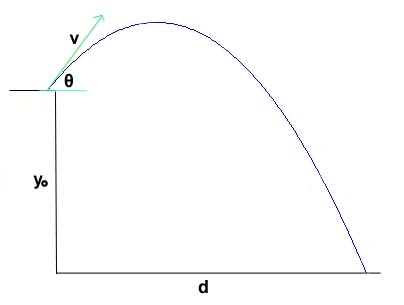
\includegraphics[scale=.6]{fig/ProjectileRange}
\caption{Range of a projectile.}
\label{fig:range}
\end{figure}

Consequently, UFFSR can show cutsets that other methods either do not consider at all (PRA, FFIP, RBD, ...), or do not consider in a consistent manner (FMEA, ...). It requires a lot of time and computational power to be performed on a large system scale. However, UFFSR can quickly gives precious information about the system risks and reliability, though the conclusions drawn need to be refined as more details are available. In this case study, we saw that the turbine explosion was a real risk to the system, and that simple measures could be taken, such as the turbines orientations and a concrete wall, in order to mitigate the risks. The analysis done is a simplified case of what UFFSR can do. Indeed, the probability of an uncoupled flow was not considered in the scenario studied, only the possibility. The probability of an uncoupled flow reaching other functions in the system is a function of the distance between the initiating event and the analyzed function $d_{i, f}$, as well as the analyzed function resistance to the incoming flow $s_{f, i}$. It can be written $P = f(d_{i, f}, s_{f, i})$. There resides the real future strength of UFFSR, once a computational framework is created.

\section{Prognostics in Early Functional Design}

More and more systems use \gls{phm} hardware to detect future failures and allow for preventive maintenance and recovery actions, automated or manual. However, the hardware is often added on after the system has been built or during the late stages of the design. In the early stages of the design, PHM is currently not seriously considered, despite the consequent impact it can have on the system failure and the subsequent design choices made. Hence, a system can be designed with unnecessary expensive redundancies which could be deprecated by PHM hardware. The earlier in the design phase a system fault is discovered, the less costly the design required modifications can be. Being able to consider prognosis in the early phases by modeling the impact of PHM hardware allow the designer to limit the costly system changes and increase the system reliability.

Probabilistic Risk Assessment (PRA) method is able to model failure detection and recovery actions, but is limited by its rigidness, time-consuming changes, and by its use in the late phases of design. FMEA or functional failure methods, such as FFDM or FFIP, are not able to model recovery actions in a dedicated framework.

The Prognostics in Early Design method proposed in this paper creates a framework that enable the use of a functional failure method in various stages of design, notably early on, coupled with PHM hardware considerations. A Bayesian network is used to compute the functional failure propagation probabilities. The optimized configuration for PHM equipment positioning is automatically given to the system designer, 
who can then decide to move forward with it or modify the system, according to the system failure probability returned by the algorithm.


\subsection{Methodology}

The methodology can be discretized into four main parts. This method is based upon a functional representation of a system as developed by Stone~\cite{stone}, augmented with \gls{sta}, the logical opposite of FTA. Four distinct databases are necessary to represent various system information. They comprise information about PHM hardware efficiency, emergent function weaknesses, impacts of function failure on subsequent linked flows quality, and tie the probability of corrective action success to each particular system function and flow. The selection and positioning of PHM hardware through the designed system is generated. The Bayesian network representing the complex system is consequently built following the framework shown in figure~\ref{fig:cptex}. A risk and reliability analysis is performed on the system. The positioning of PHM equipment can then iterately be modified to compute the best possible system configuration and supports the decision making.


\begin{figure}[H]
\centering
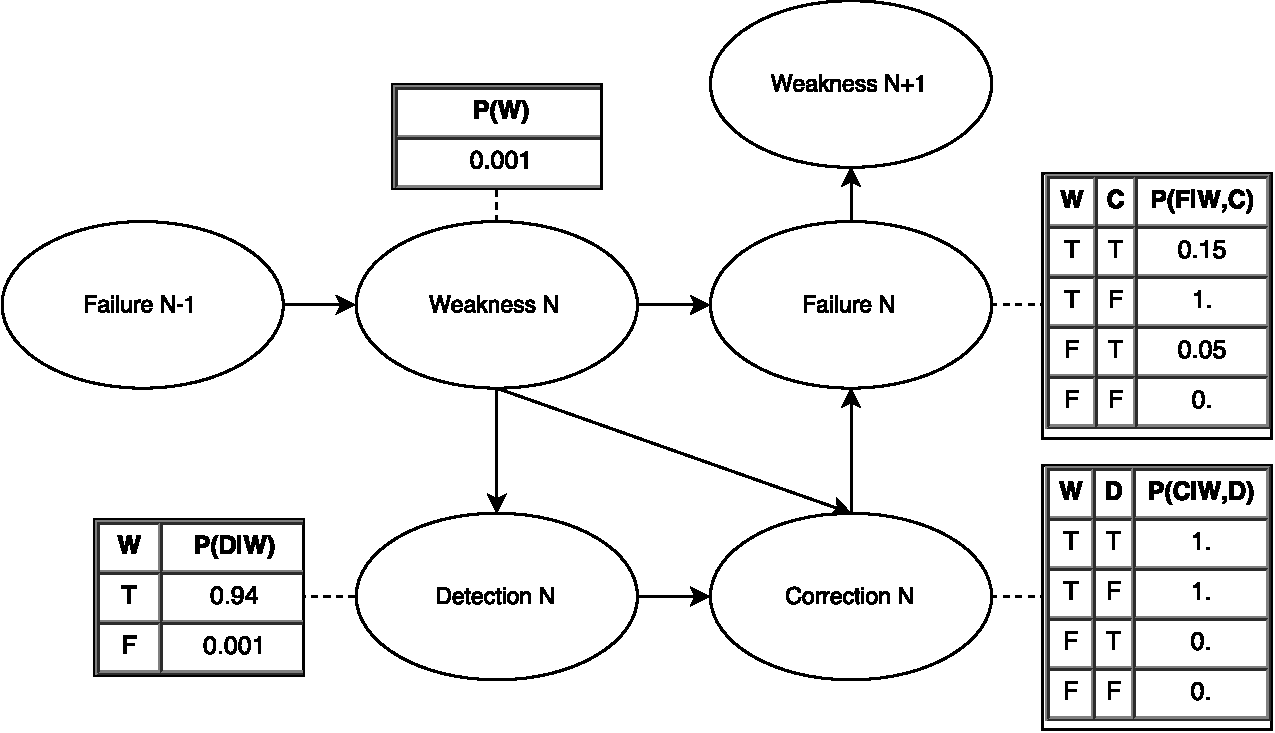
\includegraphics[scale=.6]{fig/cptex}
\caption{Example of the method prognostic bayes net.}
\label{fig:cptex}
\end{figure}


In order to illustrate the algorithm presented, a small example is given. Figure~\ref{fig:fm} presents a very simple functional model, and Figure~\ref{fig:bn_example} its translation into the proposed method model, provided each function and flow are linked to a PHM device. The interaction with the various database, $\mathscr{F}$, $\mathscr{H}$, $\mathscr{M}$, $\mathscr{P}$ and $\mathscr{W}$ is also shown in Figure~\ref{fig:bn_example}. If the designer were to force the flow $f_{12}$ not to be equipped with a PHM hardware, the nodes \textit{Detection} $f_{12}$ and \textit{Correction} $f_{12}$ would disappear from the model, along with the connections.


\begin{figure}[H]
\centering
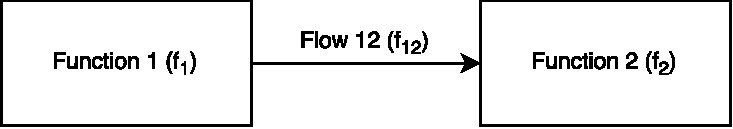
\includegraphics[scale=.5]{fig/fm}
\caption{Simple functional model.}
\label{fig:fm}
\end{figure}


\begin{figure}[H]
\centering
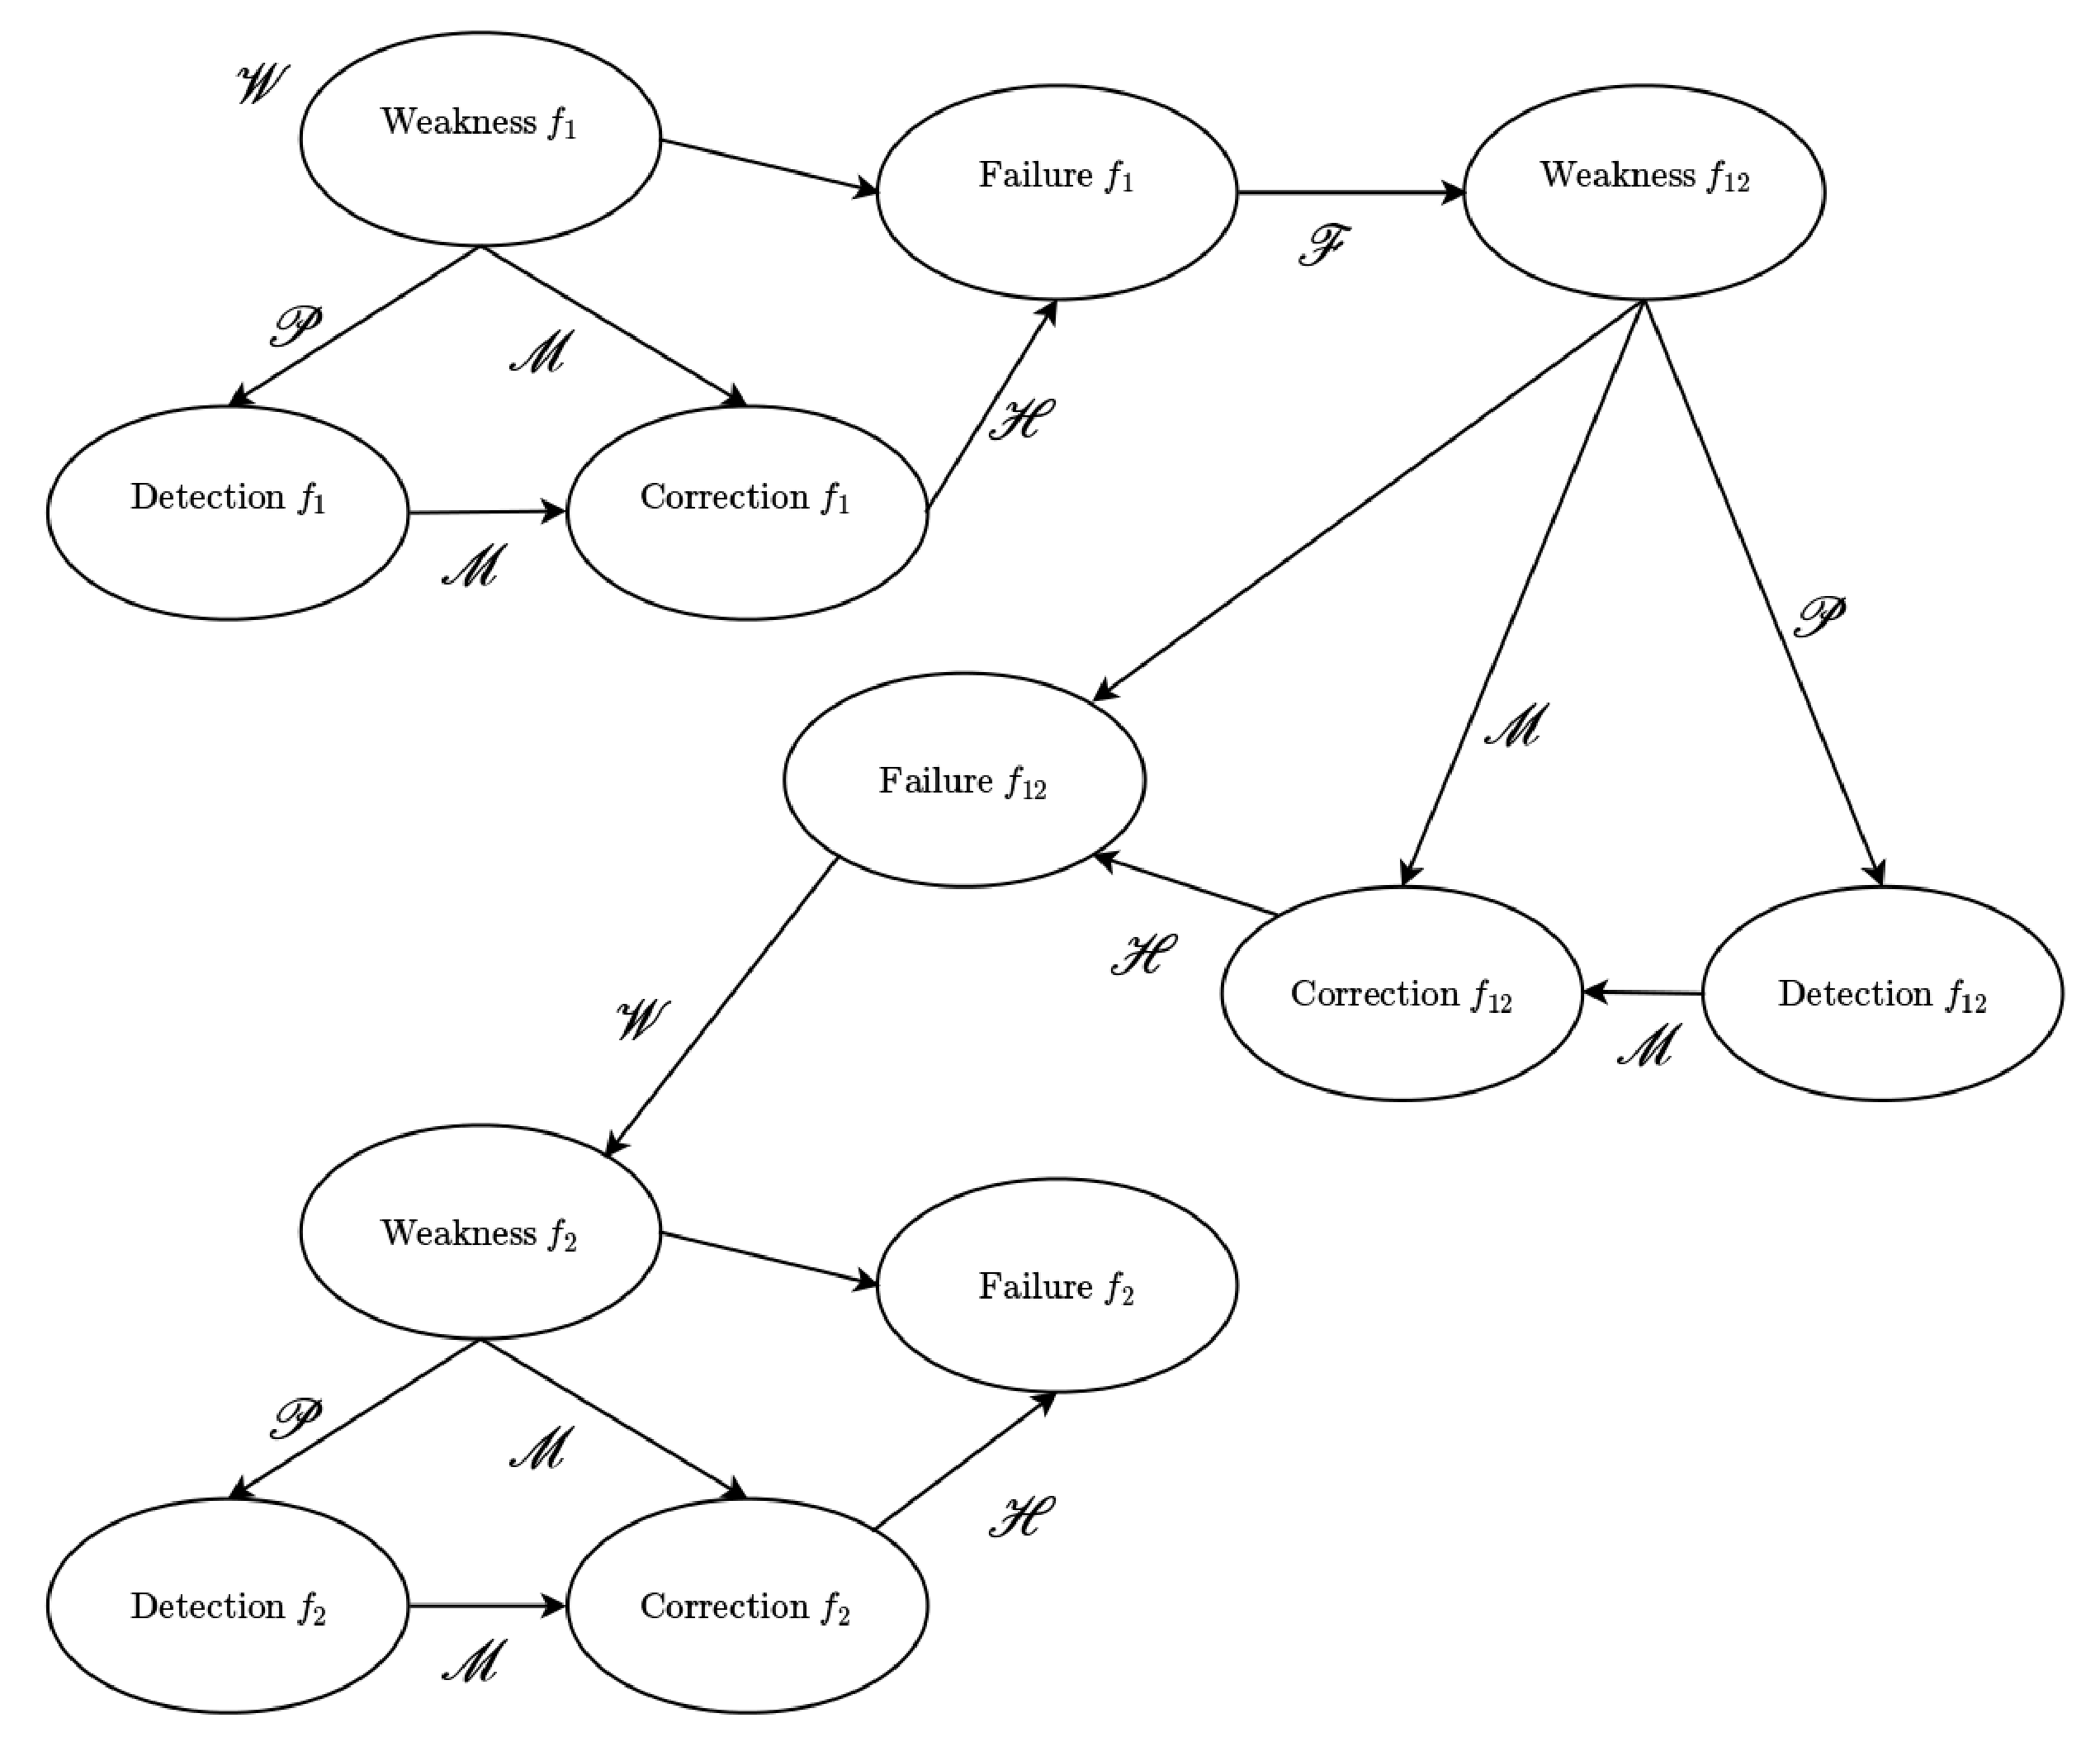
\includegraphics[scale=.3]{fig/bn_example}
\caption{Translation of a simple function model (Figure~\ref{fig:fm}) to its functional prognostic Bayesian network form.}
\label{fig:bn_example}
\end{figure}

The Bayesian network used to describe the whole system is based upon the following algorithm steps.

\textbf{Step 0}\hspace{5pt}
This step is optional. In a Bayesian network, the designer can set the states of several functions and flows. While not particularly useful to generate the risk and reliability analysis on the system during the early design phase, it can be noted that this feature can be used simultaneously as a Prognostics and Diagnostics tool during the operational lifetime of the system.


\textbf{Step 1}\hspace{5pt}
The algorithm computes the probability of a function weakness, given the observed evidence (step 0) or $\mathscr{W}$. The function weakness nodes is a binary event, meaning that it can only take one of two potential states. Consequently, either there is a weakness or the function is in a nominal state, as represented by $W$ in Equation~\ref{mat_w_func} for the function $f_1$.

\begin{equation}
  P(W_{f_1}) = \kbordermatrix{
    state  & \\
    Y & \omega_{f_1} \\
    N & \bar{\omega_{f_1}} = 1 - \omega_{f_1}
  }
\label{mat_w_func}
\end{equation}


\textbf{Step 2}\hspace{5pt}
The weakness probability associated with $f_1$ has been computed in step 1. The probability of being in a state of detection by a PHM hardware can now be calculated. Several potential states can be described to link a weakness of a function to its detection. There could effectively be a weakness, and this weakness could be detected according to the attached hardware efficiency $\varepsilon_{phm, f_1}$. The probability of this event will be noted $d_{\varepsilon, f_1}$. Alternatively, there might be no function weakness, but a false alarm is raised by the hardware according to its false alarm rate $e_{phm, f_1}$. The probability of this event will be noted $d_{e, f_1}$. The combination of these two events forms the probability of a detection.

The probability of being in the state of non detection, is trivially the complement of the probability of detection. Either the weakness is present and not detected, or there is no weakness, and no false alarm is raised.

The different probability path leading to the probability of detection are represented in Table~\ref{tab:cpt_dcf}.


\renewcommand{\arraystretch}{1.5}
\begin{table}[t] \small
\centering
\caption{Conditional probability tables for the weakness detection, correction and failure of a function $f_1$}
\label{tab:cpt_dcf}
\begin{tabular}{|c|c|c|c|c|c|}
\hline
$P(D_{f_1} | W_{f_1})$                           & Weakness $f_1$   & \multicolumn{2}{c|}{Y}                          & \multicolumn{2}{c|}{N}                \\ \hline
\multirow{2}{*}{Detection $f_1$}                 & Y                & \multicolumn{2}{c|}{$\varepsilon_{phm, f_1}$}   & \multicolumn{2}{c|}{$e_{phm, f_1}$}   \\ \cline{2-6} 
                                                 & N                & \multicolumn{2}{c|}{$1-\varepsilon_{phm, f_1}$} & \multicolumn{2}{c|}{$1-e_{phm, f_1}$} \\ \hline \hline
\multirow{2}{*}{$P(C_{f_1} | W_{f_1}, D_{f_1})$} & Weakness $f_1$   & \multicolumn{2}{c|}{Y}                          & \multicolumn{2}{c|}{N}                \\ \cline{2-6} 
                                                 & Detection $f_1$  & Y                        & N                    & Y                   & N               \\ \hline
\multirow{2}{*}{Correction $f_1$}                & Y                & $\gamma_{f_1}$           & $\mu_{f_1}$          & $\gamma_{f_1}$      & $\mu_{f_1}$     \\ \cline{2-6} 
                                                 & N                & $1-\gamma_{f_1}$         & $1-\mu_{f_1}$        & $1-\gamma_{f_1}$    & $1-\mu_{f_1}$   \\ \hline \hline
\multirow{2}{*}{$P(F_{f_1} | W_{f_1}, C_{f_1})$} & Weakness $f_1$   & \multicolumn{2}{c|}{Y}                          & \multicolumn{2}{c|}{N}                \\ \cline{2-6} 
                                                 & Correction $f_1$ & Y                        & N                    & Y                   & N               \\ \hline
\multirow{2}{*}{Failure $f_1$}                   & Y                & $1-\rho_{f_1}$           & 1                    & $\beta_{f_1}$       & 0               \\ \cline{2-6} 
                                                 & N                & $\rho_{f_1}$             & 0                    & $1-\beta_{f_1}$     & 1               \\ \hline
\end{tabular}
\end{table}

Given the function weakness probability, the detection conditional probability matrix $P(D_{f_1} | W_{f_1})$ obtained is displayed in Equation~\ref{prob_d_func}.

\begin{equation}
  P(D_{f_1} | W_{f_1}) = \kbordermatrix{
    state  & \\
    Y & d_{\varepsilon, f_1} + d_{e, f_1} \\
    N & d'_{\varepsilon, f_1} + d'_{e, f_1}
  }
\label{prob_d_func}
\end{equation}
Where:
\begin{conditions}
d_{\varepsilon, f_1} & $\omega_{f_1}\varepsilon_{phm, f_1}$ \\
d_{e, f_1} & $(1-\omega_{f_1})e_{phm, f_1}$ \\
d'_{\varepsilon, f_1} & $\omega_{f_1}(1-\varepsilon_{phm, f_1})$ \\
d'_{e, f_1} & $(1-\omega_{f_1})(1-e_{phm, f_1})$
\end{conditions}


This step is performed if and only if the function of interest is equipped with a PHM hardware. Indeed, if a PHM hardware is not attached to the function, the detection is trivially non-existent, implying $\varepsilon_{phm, f_1} = 0$ and $e_{phm, f_1} = 0$. Entering these numbers in Equation~\ref{prob_d_func}, we obtain the relation~\ref{prob_d_func_nophm}.

\begin{equation}
  P(D_{f_1} | W_{f_1}) = \kbordermatrix{
    state  & \\
    Y & 0 \\
    N & 1
  }
\label{prob_d_func_nophm}
\end{equation}


\textbf{Step 3}\hspace{5pt}
The weakness probability and the detection probability have been computed respectively in step 1 and step 2. This third step estimates the probability of a corrective action being attempted. The potential scenarii leading to the corrective action are treated by the conditional probability table presented in Table~\ref{tab:cpt_dcf}. In the case of an actual weakness, the detector could detect the weakness ($d_{\varepsilon, f_1}$). Then, the maintenance team is sent to repair according to a decision probability $\gamma_{f_1}$ given by $\mathscr{M}$. Alternatively, the weakness is not detected ($d'_{\varepsilon, f_1}$) but a scheduled non required maintenance is done on the function, according to a probability $\mu_{f_1}$ also given by $\mathscr{M}$. The combination of these two events translate to a probability noted $c_{\omega, f_1}$. Maintenance can also be carried out on the function if no weakness actually happened. This event is true if a false alarm ($d_{e, f_1}$) caused the maintenance team to mobilize or if a scheduled non required maintence is performed. These two events can be combined to obtain a probability noted $c_{\bar{\omega}, f_1}$. Finally, the corrective action probability can be calculated by combining $c_{\omega, f_1}$ with $c_{\bar{\omega}, f_1}$.

Considering the fact that the corrective action is a binary event, the probability of no corrective action being carried out is trivially the complement of the probability that a corrective action is performed.


Given the function weakness probability $P(W_{f_1})$ and the detection probability matrice $P(D_{f_1} | W_{f_1})$, the conditional corrective action matrice obtained is displayed in Equation~\ref{prob_c_func}.

\begin{equation}
  P(C_{f_1} | W_{f_1}, D_{f_1}) = \kbordermatrix{
    state  & \\
    Y & c_{\omega, f_1} + c_{\bar{\omega}, f_1} \\
    N & c'_{\omega, f_1} + c'_{\bar{\omega}, f_1}
  }
\label{prob_c_func}
\end{equation}
Where:
\begin{conditions}
c_{\omega, f_1} & $d_{\varepsilon, f_1}\gamma_{f_1} + d'_{\varepsilon, f_1}\mu_{f_1}$ \\
c_{\bar{\omega}, f_1} & $d_{e, f_1}\gamma_{f_1} + d'_{e, f_1}\mu_{f_1}$ \\
c'_{\omega, f_1} & $d_{\varepsilon, f_1}(1-\gamma_{f_1}) + d'_{\varepsilon, f_1}(1-\mu_{f_1})$ \\
c'_{\bar{\omega}, f_1} & $d_{e, f_1}(1-\gamma_{f_1}) + d'_{e, f_1}(1-\mu_{f_1})$
\end{conditions}


\textbf{Step 4}\hspace{5pt}
Based on the weakness probability and the corrective action probability, calculated respectively in step 1 and step 3, the algorithm computes the probability of the function failure using the conditional probability table displayed in Table~\ref{tab:cpt_dcf}. In the case of an actual weakness, the path leading to a failure can be that no corrective action was performed ($c'_{\omega, f_1}$), or that a corrective action was performed ($c_{\omega, f_1}$) but was unsuccessful, according to the $\rho_{f_1}$ value given in $\mathscr{H}$. Alternatively, a function can fail if there was no weakness but a corrective action was still performed ($c_{\bar{\omega}, f_1}$) and generated a function failure according to the mishandling probability $\beta_{f_1}$ given by $\mathscr{H}$. The failure probability of $f_1$ is obtained by combining these different scenarii.

The probability that the function does not fail is obtained if a weakness was present but was corrected following the $\rho_{f_1}$ value, or no weakness was present and either no action were perforned or the performed action did not fail the function, according to the mishandling probability $\beta_{f_1}$. This corresponds to the complement of the probability of failure.


Given the function weakness probability $P(W_{f_1})$ and the correction probability matrice $P(C_{f_1} | W_{f_1}, D_{f_1})$, the conditional failure matrice obtained is displayed in Equation~\ref{prob_f_func}.

\begin{equation}
  P(F_{f_1} | W_{f_1}, C_{f_1}) = \kbordermatrix{
    state  & \\
    Y & f_{f_1} \\
    N & f'_{f_1}
  }
\label{prob_f_func}
\end{equation}
Where:
\begin{conditions}
f_{f_1} & $c_{\omega, f_1}(1-\rho_{f_1}) + c'_{\omega, f_1} + c_{\bar{\omega}, f_1}\beta_{f_1}$ \\
f'_{f_1} & $c_{\omega, f_1}(\rho_{f_1}) + c'_{\bar{\omega}, f_1} + c_{\bar{\omega}, f_1}(1-\beta_{f_1})$
\end{conditions}



\textbf{Step 5}\hspace{5pt}
A function failure can be linked to different outgoing flow quality. The flow quality represents a state of weakness and is modeled by a $s$-event. A $s$-event is an event that can take four distinct states of flow quality. The quality of a flow can be categorized as failed ($\lambda_f$), of low concern ($\lambda_l$), of high concern ($\lambda_h$), or nominal ($\lambda_n$). The algortihm considers that the quality of a flow cannot spontaneously change without an impact on the last function acting on it. This represents one of the simulation limitation, as discussed previously. Indeed, it does not allow for the treatment of failure flows going through a function without failing it.

$\mathscr{F}$ contains the detailed data for each specific function-flow connection. The probability of weakness $P(W_{f_{12}} | F_{f_1})$ is displayed in Equation~\ref{prob_ftow_func}.

\begin{equation}
  P(W_{f_{12}} | F_{f_1}) = \kbordermatrix{
    state  & \\
    f & w_{f, f_{12}} \\
    l & w_{l, f_{12}} \\
    h & w_{h, f_{12}} \\
    n & w_{n, f_{12}}
  }
\label{prob_ftow_func}
\end{equation}
Where:
\begin{conditions}
  w_{f, f_{12}} & $\lambda_{f, f_{12}}f_{f_1}$ \\
  w_{l, f_{12}} & $\lambda_{l, f_{12}}f_{f_1}$ \\
  w_{h, f_{12}} & $\lambda_{h, f_{12}}f_{f_1}$ \\
  w_{n, f_{12}} & $f_{f_1} + f'_{f_1} - \sum_{i \in [f, h, l]}f_{f_1}\lambda_i$
\end{conditions}


\textbf{Step 6}\hspace{5pt}
The weakness probability of $f_{12}$ has been computed in step 5. The probability of a detection can now be calculated. Similarily to step 2, several potential states can be described to link a weakness of a flow to its detection. There could effectively be a flow quality weakness, which is detected according to the attached hardware efficiencies. The hardware efficiencies for a flow are given for the three states of degraded operation, low concern ($\varepsilon_{phm, l, f_{12}}$), high concern ($\varepsilon_{phm, h, f_{12}}$) and failed ($\varepsilon_{phm, f, f_{12}}$). The probability of a scenario in which a weakness is present and detected will be noted $d_{\varepsilon_i, f_{12}}$, for $i \in [f, l, h]$. Alternatively, a detection might occur if there is no flow weakness, but a false alarm is raised by the hardware according to its false alarm rate $e_{phm, f_{12}}$. The probability of this event will be noted $d_{e, f_{12}}$. The combination of these two events forms the probability of a detection. This can be seen in Table~\ref{tab:cpt_dcf_flow}.

The probability of not having a detection is the complement of the probability of having a detection. Indeed, if the flow quality is not nominal, the detector might fail to detect it, with a probability depending on its efficiency. If the flow quality is nominal, the detector can also not signal any issue, based on its false alarm rate.

\renewcommand{\arraystretch}{1.5}
\begin{table}[t] \tiny
\centering
\caption{Conditional probability tables for the weakness detection, correction and failure of a flow $f_{12}$}
\label{tab:cpt_dcf_flow}
\begin{tabular}{|c|c|c|c|c|c|c|c|c|c|}
\hline
$P(D_{f_{12}} | W_{f_{12}})$                              & Weakness $f_{12}$   & \multicolumn{2}{c|}{Failed}                           & \multicolumn{2}{c|}{Low concern}                      & \multicolumn{2}{c|}{High concern}                     & \multicolumn{2}{c|}{Nominal}                 \\ \hline
\multirow{2}{*}{Detection $f_{12}$}                       & Y                   & \multicolumn{2}{c|}{$\varepsilon_{phm, f, f_{12}}$}   & \multicolumn{2}{c|}{$\varepsilon_{phm, l, f_{12}}$}   & \multicolumn{2}{c|}{$\varepsilon_{phm, h, f_{12}}$}   & \multicolumn{2}{c|}{$e_{phm, f_{12}}$}       \\ \cline{2-10} 
                                                          & N                   & \multicolumn{2}{c|}{$1-\varepsilon_{phm, f, f_{12}}$} & \multicolumn{2}{c|}{$1-\varepsilon_{phm, l, f_{12}}$} & \multicolumn{2}{c|}{$1-\varepsilon_{phm, h, f_{12}}$} & \multicolumn{2}{c|}{$1-e_{phm, f_{12}}$}     \\ \hline \hline
\multirow{2}{*}{$P(C_{f_{12}} | W_{f_{12}}, D_{f_{12}})$} & Weakness $f_{12}$   & \multicolumn{2}{c|}{Failed}                           & \multicolumn{2}{c|}{Low concern}                      & \multicolumn{2}{c|}{High concern}                     & \multicolumn{2}{c|}{Nominal}                 \\ \cline{2-10} 
                                                          & Detection $f_{12}$  & Y                           & N                       & Y                           & N                       & Y                           & N                       & Y                      & N                   \\ \hline
\multirow{2}{*}{Correction $f_{12}$}                      & Y                   & $\gamma_{f, f_{12}}$        & $\mu_{f, f_{12}}$       & $\gamma_{l, f_{12}}$        & $\mu_{l, f_{12}}$       & $\gamma_{h, f_{12}}$        & $\mu_{h, f_{12}}$       & $\gamma_{n, f_{12}}$   & $\mu_{n, f_{12}}$   \\ \cline{2-10} 
                                                          & N                   & $1-\gamma_{f, f_{12}}$      & $1-\mu_{f, f_{12}}$     & $1-\gamma_{l, f_{12}}$      & $1-\mu_{l, f_{12}}$     & $1-\gamma_{h, f_{12}}$      & $1-\mu_{h, f_{12}}$     & $1-\gamma_{n, f_{12}}$ & $1-\mu_{n, f_{12}}$ \\ \hline \hline
\multirow{2}{*}{$P(F_{f_{12}} | W_{f_{12}}, C_{f_{12}})$} & Weakness $f_{12}$   & \multicolumn{2}{c|}{Failed}                           & \multicolumn{2}{c|}{Low concern}                      & \multicolumn{2}{c|}{High concern}                     & \multicolumn{2}{c|}{Nominal}                 \\ \cline{2-10} 
                                                          & Correction $f_{12}$ & Y                           & N                       & Y                           & N                       & Y                           & N                       & Y                      & N                   \\ \hline
\multirow{2}{*}{Failure $f_{12}$}                            & Y                   & $1-\rho_{f, f_{12}}$        & 1                       & $1-\rho_{l, f_{12}}$        & 1                       & $1-\rho_{h, f_{12}}$        & 1                       & $\beta_{f_{12}}$       & 0                   \\ \cline{2-10} 
                                                          & N                   & $\rho_{f, f_{12}}$          & 0                       & $\rho_{l, f_{12}}$          & 0                       & $\rho_{h, f_{12}}$          & 0                       & $1-\beta_{f_{12}}$     & 1                   \\ \hline
\end{tabular}
\end{table}

Given the flow weakness probability, the detection conditional probability matrice $P(D_{f_{12}} | W_{f_{12}})$ obtained is displayed in Equation~\ref{prob_d_flow}.


\begin{equation}
  P(D_{f_{12}} | W_{f_{12}}) = \kbordermatrix{
    state  & \\
    Y & \sum_{i \in [f, h, l]} d_{\varepsilon_i, f_{12}} + d_{e, f_{12}} \\
    N & \sum_{i \in [f, h, l]} d'_{\varepsilon_i, f_{12}} + d'_{e, f_{12}}
  }
\label{prob_d_flow}
\end{equation}
Where:
\begin{conditions}
d_{\varepsilon_i, f_{12}} & $\omega_{i, f_{12}}\varepsilon_{phm, i, f_{12}}$ \\
d_{e, f_{12}} & $\omega_{n, f_{12}} e_{phm, f_{12}}$ \\
d'_{\varepsilon_i, f_{12}} & $\omega_{i, f_{12}}(1-\varepsilon_{phm, i, f_{12}})$ \\
d'_{e, f_{12}} & $\omega_{n, f_{12}}(1-e_{phm, f_{12}})$
\end{conditions}

This step is performed if and only if the function of interest is equipped with a PHM hardware. Indeed, if a PHM hardware is not attached to the function, the detection is trivially in a false state.


\textbf{Step 7}\hspace{5pt}
The flow weakness probability and the detection probability have been computed respectively in step 5 and step 6. This next step estimates the probability of a corrective action being attempted. The potential scenario leading to the corrective action are treated by the conditional probability table presented in Table~\ref{tab:cpt_dcf_flow}. In the case of an actual weakness, the detector could detect the weakness according to the corresponding hardware efficiency for each flow quality ($d_{\varepsilon_i, f_{12}}$ for $i \in [f, l, h]$). If the event is detected, the maintenance team is sent to repair according to a decision probability $\gamma_{i, f_{12}}$ for $i \in [f, l, h]$, based on the team management and the detected flow quality weakness. The decision probability is given by $\mathscr{M}$. Alternatively, the weakness could be undetected ($d'_{\varepsilon_i, f_{12}}$ for $i \in [f, l, h]$) but a scheduled non required maintenance could be performed on the system which would impact the flow, according to a probability $\mu_{f_{12}}$ also given by $\mathscr{M}$. The combination of these two events translates to a probability noted $c_{\omega, i, f_{12}}$ for $i \in [f, l, h]$. Maintenance can also be carried out on the system, with a direct impact on the flow $f_{12}$ if no weakness actually happened. This event is true if a false alarm ($d_{e, f_{12}}$) caused the maintenance team to mobilize or if a scheduled non required maintence is performed. These two events can be combined to obtain a probability noted $c_{\bar{\omega}, f_{12}}$. Finally, the corrective action probability can be calculated by combining $c_{\omega, i, f_{12}}$ with $c_{\bar{\omega}, f_{12}}$ for $i \in [f, l, h]$.

The probability that no corrective action is attempted is the complement of the probability that a corrective action is carried out.


Given the function weakness probability $P(W_{f_{12}} | F_{f_1})$ and the detection probability matrice $P(D_{f_{12}} | W_{f_{12}})$, the conditional corrective action matrice obtained is displayed in Equation~\ref{prob_c_flow}.

\begin{equation}
  P(C_{f_{12}} | W_{f_{12}}, D_{f_{12}}) = \kbordermatrix{
    state  & \\
    Y & \sum_{i \in [f, l, h, n]}c_{\omega_i, f_{12}} \\
    N & \sum_{i \in [f, l, h, n]}c'_{\omega_i, f_{12}} 
  }
\label{prob_c_flow}
\end{equation}
Where, for $i \in [f, l, h]$:
\begin{conditions}
c_{\omega_i, f_{12}} & $d_{\varepsilon_i, f_{12}}\gamma_{i, f_{12}} + d'_{\varepsilon_i, f_{12}}\mu_{f_{12}}$ \\
c_{\omega_n, f_{12}} & $d_{e, f_{12}}\gamma_{n, f_{12}} + d'_{e, f_{12}}\mu_{f_{12}}$ \\
c'_{\omega_i, f_{12}} & $d_{\varepsilon_i, f_{12}}(1-\gamma_{i, f_{12}}) + d'_{\varepsilon_i, f_{12}}(1-\mu_{f_{12}})$ \\
c'_{\omega_n, f_{12}} & $d_{e, f_{12}}(1-\gamma_{n, f_{12}}) + d'_{e, f_{12}}(1-\mu_{f_{12}})$
\end{conditions}



\textbf{Step 8}\hspace{5pt}
Based on the flow weakness probability and the corrective action probability, calculated respectively in step 5 and step 7, the algorithm computes the probability of the flow failure using the conditional probability table displayed in Table~\ref{tab:cpt_dcf_flow}.

In the case of an actual weakness, either of low concern, of high concern, or failed, the path leading to a failure can be that no corrective action was performed $\left(\sum_{i \in [f, l, h]}c'_{\omega_i, f_{12}}\right)$, or that a corrective action was performed $\left(\sum_{i \in [f, l, h]}c_{\omega_i, f_{12}}\right)$ but was unsuccessful, according to the $\rho_{i, f_{12}}$ values for $i \in [f, l, h]$ given in $\mathscr{H}$. Alternatively, the flow can fail if there was no weakness but a corrective action was still performed on the system ($c_{\omega_n, f_{12}}$) and generated a function failure according to the mishandling probability $\beta_{f_{12}}$ given by $\mathscr{H}$.


Given the function weakness probability $P(W_{f_1})$ and the correction probability matrice $P(C_{f_1} | W_{f_1}, D_{f_1})$, the conditional failure matrice obtained is displayed in Equation~\ref{prob_f_flow}.

\begin{equation}
  P(F_{f_{12}} | W_{f_{12}}, C_{f_{12}}) = \kbordermatrix{
    state  & \\
    Y & f_{f_{12}} \\
    N & f'_{f_{12}}
  }
\label{prob_f_flow}
\end{equation}
Where:
\begin{conditions}
f_{f_{12}} & $c_{\omega_n, f_{12}}\beta_{ f_{12}} + \sum_{i \in [f, l, h]} c_{\omega_i, f_{12}} (1-\rho_{i, f_{12}}) + c'_{\omega_i, f_{12}}$ \\
f'_{f_{12}} & $c_{\omega_n, f_{12}}(1-\beta_{ f_{12}}) + c'_{\omega_n, f_{12}} + \sum_{i \in [f, l, h]} c_{\omega_i, f_{12}} \rho_{i, f_{12}}$
\end{conditions}


If the next Bayesian node in the model is a logical gate, the algorithm goes to step 9-b. Else, it goes back to step 9-a.



\textbf{Step 9-a}\hspace{5pt}
A failed flow is considered to fail a receiving function, since the function will not be able to perform its task without a necessary flow. The failure probability obtained in step 8 for the flow is thus passed fully to the next function in the model. The emergent weakness of the next function in the model is also considered. Consequently, given $P(F_{f_{12}} | W_{f_{12}}, C_{f_{12}})$, the weakness probability seen by the next function is displayed in the conditional failure matrice in Equation~\ref{prob_w_func_2}.


\begin{equation}
  P(W_{f_{2}} | F_{f_{12}}) = \kbordermatrix{
    state  & \\
    Y & f_{f_{12}} + \omega_{f_{2}} \\
    N & f'_{f_{12}} - \omega_{f_{2}}
  }
\label{prob_w_func_2}
\end{equation}

The algorithm returns to step 1.


\textbf{Step 9-b}\hspace{5pt}
Logical gates can combine several flows and compute the next function weakness associated. Consider another flow, $f_{32}$, supplying a redundant flow to function $f_2$. An OR-gate is placed in the model, so that only one flow, $f_{12}$ or $f_{32}$ is needed for function $f_2$ to operate nominally.

The probability that the flow failures propagate through the gate $g_{12, 32}$ to the next function weakness, $P(F_{f_2} | F_{f_{12}}, F_{f_{32}})$, is explicited in Equation~\ref{gateor}.

\begin{equation}
\begin{aligned}
  P(F_{g_{12, 32}} | F_{f_{12}}, F_{f_{23}}) = \\ \kbordermatrix{
    state  & \\
    Y & f_{f_{12}} f_{f_{32}} \\
    N & f'_{f_{12}} f_{f_{32}} + f_{f_{12}} f'_{f_{32}} + f'_{f_{12}} f'_{f_{32}}
  }
\end{aligned}
\label{gateor}
\end{equation}


The gate failure probability becomes the new flow failure probability. The algorithm returns to step 9-a.

\subsection{Application to the case study}

The existing automatic tools to compute the optimized combination of PHM hardware in the system and the associated probability of failure is not yet able to run the simulation of a quite large functional models such as the one presented in figure~\ref{fig:fbed} on a local computer in a reasonable amount of time. Work is ongoing to parallelize the algortihm and optimize its runtime. In order to illustrate part of the method, a subset of the system will be considered. The failure of the turbine, as studied in the work relative to FFIP and UFFSR, is going to be considered. Two different sensors can be used to detect a weakness of the function. The change in the final probability of failure after taking into account the PHM hardware will be computed.

Two different kind of sensors could be used to detect a potential failure of the function fo interest. In our case, we will consider a sensor giving the rotation speed of the turbine ($S$) and a sensor giving the vapor quality and flow ($Q$). $S$ is taken as having a $85\%$ chance of detecting an anomaly leading to a function failure. A false alarm rate of $0.001$ is imagined. Alternatively, $Q$ has a $98\%$ chance of detecting an anomaly and a false alarm rate of $0.1$.

Table~\ref{tab:astrid_det} shows the chosen parameters.

\begin{table}[t]
\centering
\caption{Detectors considered}
\label{tab:astrid_det}
\begin{tabular}{|c|c|c|}
\hline
Detector & $\varepsilon$ & $e$   \\ \hline
$S$      & 0.80          & 0.001 \\ \hline
$Q$      & 0.98          & 0.1   \\ \hline
\end{tabular}
\end{table}

An "ideal" management is considered, based uniquely on PHM hardware data. Consequently, $\gamma = 1$ and $\mu = 0$. This implies that a maintenance team is sent if and only if a detector indicates a potential weakness.

After detection of an anomaly, the repair success is computed according to \gls{hra}. In our case, we will consider that should a weakness be detected on the function \textit{Channel - Guide - Rotate} representing the turbine, the following algorithm should be followed to obtain the repair success probability. The assumptions made are presented in table~\ref{tab:hra}. The human error probability (HEP) is defined from the combination of the Performance Shaping Factors ($PSF_c$) corresponding to different essential parts of the maintenance success such as stress factor or task complexity. It follows Equation~\ref{eq:hra}. $NHEP$ is defined in HRA as being equal to 0.001 for action-based maintenance. The mishandling probability is computed from $PSF_c$ disregarding the time component.

\begin{equation}
HEP = \frac{NHEP * PSF_c}{NHEP * (PSF_c-1) + 1}
\label{eq:hra}
\end{equation}

\begin{table}[t]
\centering
\caption{Estimates of the different HRA categories}
\label{tab:hra}
\begin{tabular}{|c|c|}
\hline
Category         & Level                          \\ \hline \hline
available time   & Time available = time required \\ \hline
stress           & Nominal                        \\ \hline
complexity       & Nominal                        \\ \hline
human training   & Low                            \\ \hline
procedures       & Insufficient information       \\ \hline
ergonomics       & Nominal                        \\ \hline
fitness for duty & Nominal                        \\ \hline
processes        & Good                           \\ \hline
\end{tabular}
\end{table}

Consequently, we can compute $\rho = 0.985$ and $\beta = 0.0015$.

Using these information, it is now possible to compute the impact of a detector on the probability of failure of the function of interest. We will consider an initial probability of weakness of 1, in order to compute directly the impact of the prognostics in early design method. The probability of failure is reduced to 0.035 using $Q$ and 0.21 using $S$. The higher false alarm rate is not a  big enough issue to make up for the efficiency difference. This is due to the fact that the repair or corrective action is considered simple. We consequently consider that the probability of failure of this function is lowered by almost two orders of magnitudes. This translates to the subsequent FFIP analysis of the system, lowering the probability of failure of the initiating event.

A more detailed analysis of several functions and sensors accross the system is performed. The results can be seen in table~\ref{}.

This demonstrates a small part of what this method can actually accomplish, seeing as it is not limited to one function or flow, and that it can attribute sensors to potentially every function or flow in the model. A more detailed case study, on a simplified pressurized water reactor design, is performed in~\cite{lher2016}.

Taking into account Prognostics and Health Management systems early in the design can reduce cost, by avoiding costly and redundancies and using the strength of PHM instead.


